\documentclass[]{IEEEtran}

\usepackage[italian]{babel}
\usepackage{graphicx}
\usepackage{float}
\usepackage[export]{adjustbox}
\usepackage{dirtree}
\usepackage{hyperref}
\usepackage{tikz}

\graphicspath{{figures/}} 	

\newcommand*\circled[1]{\tikz[baseline=(char.base)]{\node[shape=circle,draw,inner sep=2pt] (char) {#1};}}

\title{Sparse Matrix Transposition for GPUs}
\author{Massimiliano Incudini - VR433300\\Michele Penzo - VR439232}

\begin{document}
\maketitle

\begin{abstract}
	L'obiettivo principale di questo progetto è stato quello di implementare alcune metodologie proposte per effettuare \textit{Sparse Matrix Transposition} su \textit{Gpu}.
	Sono stati analizzati alcuni algoritmi, descritti in sezione~\ref{metodologie}, partendo dall'algoritmo seriale, passando a cuSPARSE per finire con l'implementazione degli algoritmi descritti in~\cite{parallelTrans}.
	Infine vengono esposti i risultati e tratte le conclusioni.
\end{abstract}


\section{Introduzione}
\label{introduzione}
	% problema e motivazioni
	Sempre più applicazioni computazionali in ambito scientifico necessitano di algoritmi che compiano operazioni che si possano applicare su matrici sparse. Si parla di semplici operazioni di algebra lineare, di moltiplicazione o di calcolo della trasposta come in questo caso.\newline
	Il problema analizzato, quello della trasposizione di matrici, si presta bene al calcolo parallelo per aumentarne l'efficienza. Verranno quindi mostrate le basi per la rappresentazione, i problemi riscontrati durante lo sviluppo e analizzati alcuni algoritmi per il calcolo su \textit{Gpu}.\newline


\section{Rappresentazione delle matrici}
\label{rappresentazione}
	Una matrice sparsa non è altro che una matrice i cui valori sono per la maggior parte uguali a zero. La matrice in formato classico necessita di una quantità di memoria minima di $ m $x$ n $ elementi, ma essendo l'obiettivo quello di lavorare su matrici sparse non è stato necessario e utile memorizzare la matrice in formato denso.\newline
	Per rappresentare in modo efficace le matrici sparse senza troppo utilizzo di memoria sono state quindi introdotte ed utilizzate delle forme di rappresentazione matriciale che permettono il salvataggio di dati utilizzando quantitativi di memoria inferiori.\newline
	Di seguito vengono spiegate le due metodologie da noi utilizzate.
	
	\subsection{Formato Csr}
	\label{csr}
	Il \textit{compressed sparse row} è una rappresentazione di una matrice $ M $ basata su tre array monodimensionali, che rispettivamente contengono:
	\begin{enumerate}
		\item \textit{V}: i valori \textit{nnz},
		\item \textit{COL\_INDEX}: gli indici delle colonne dove si trovano gli elementi \textit{nnz},
		\item \textit{ROW\_INDEX}: ha un elemento per ogni riga della matrice e rappresenta l'indice in $ V $ dove comincia la riga data.
	\end{enumerate}
	I primi due array sono di dimensione \textit{nnz}, mentre il terzo array è al massimo di dimensione $ m $.
	
	\subsection{Formato Csc}
	\label{csc}
 	Questa metodologia per la rappresentazione è simile alla sopra citata \textit{Csr}, a differenza che i valori vengono letti prima per colonna. Di conseguenza, un indice di riga viene memorizzato per ogni valore e i puntatori di colonna vengono memorizzati.
 	
	\subsection{Da Csr a Csc}
	\label{csr-to-csc}
 	Per il problema della trasposta di matrice è stato quindi utile introdurre entrambe le rappresentazioni. Infatti, ogni algoritmo  descritto in sezione~\ref{metodologie}, necessita di sei array per effettuare il calcolo della trasposta e ritornare l'output in modo corretto. Abbiamo quindi:
 	\begin{itemize}
 		\item in input il formato \textit{Csr}: csrRowPtr, csrColIdx, csrVal;
 		\item in output il formato \textit{Csc}: cscColPtr, cscRowIdx, cscVal.	
 	\end{itemize}
 	In base a come vengono create le matrici, se in modo casuale oppure se lette da file, vengono effettutate delle operazioni preliminari descritte dalla procedure in sezione~\ref{procedure} che portano ad ottenere gli array in input e in output nel formato corretto per effettuarne il controllo di correttezza.\newline
	
	% TODO disegnino fatto meglio
	\begin{figure}[H]
		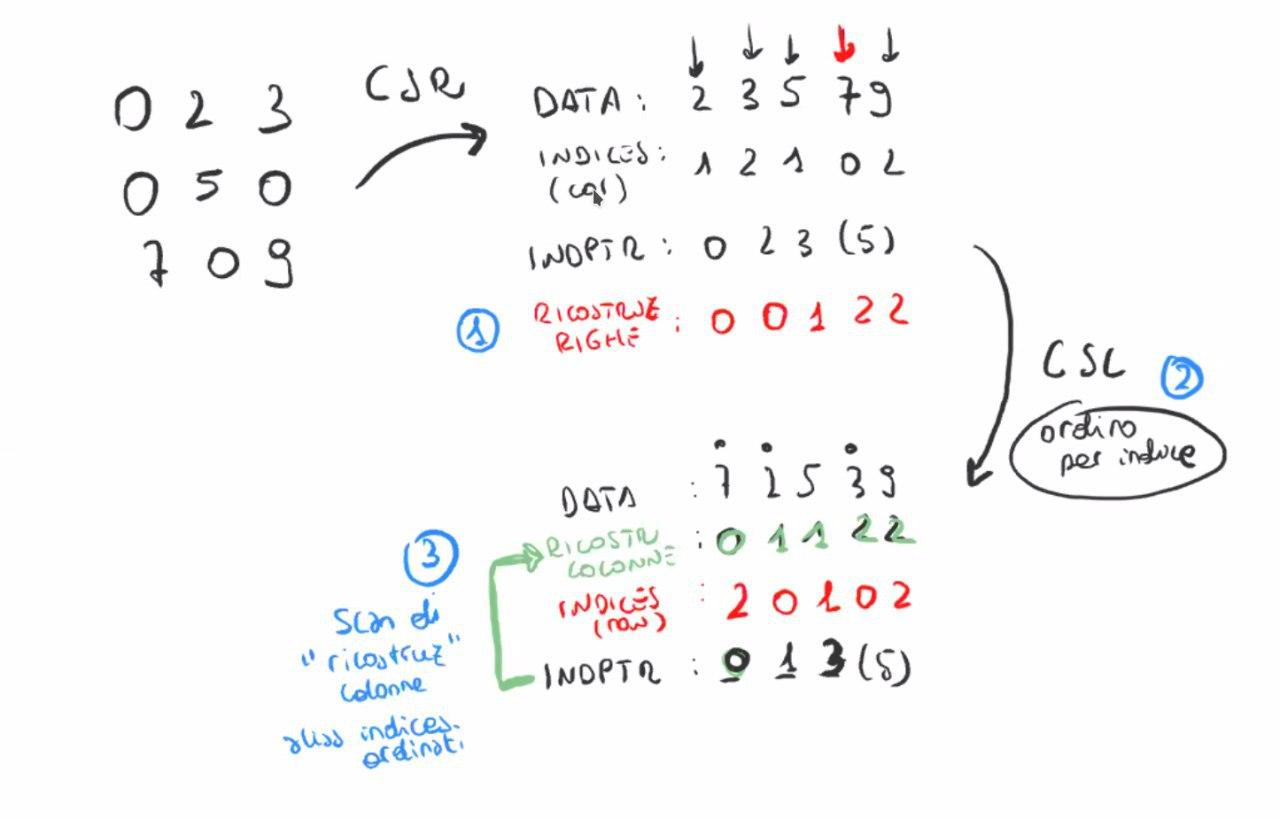
\includegraphics[scale=0.25]{csr-to-csc.jpg}
		\caption{Esempio di trasformazione da formato Csr a Csc.}
	\end{figure}

	
\section{Struttura dell'implementazione} 
\label{struttura}
	L'implementazione è stata sviluppata utilizzando come supporto il tool \textit{Git}. È stata creata una repository, descritta nella sezione successiva, per poter controllare in modo efficiente lo svilupparsi del progetto. 
	% TODO sistemare newpage
	\newpage
	\subsection{Struttura delle directory}
	La struttura delle direcotry è rispecchiata nel seguente schema:
	\dirtree{%
		.1 root.
			.2 doc.
				.3 {report\_aa.$ * $}.				
			.2 code.
				.3 {matrices}.
					.4 {$ *$.mtx }.
				.3 {include}.
					.4 {matrix.hh}.
					.4 {procedures.hh}.
					.4 {transposer.hh}.
					.4 {Timer.$ * $}.
					.4 {utilities.hh}.
				.3 {src}.
					.4 {all cuda procedures..}.
					.4 {transposer.cu}.
					.4 {main.cu}.
				.3 {test}.	
					.4 {test\_main.cu}.
				.3 Makefile.			
			.2 README.md.
	}
	\mbox{}

	Il file \texttt{matrix.hh} è composto da due classi con i relativi campi e metodi che si occupa della:
	\begin{enumerate}
		\item costruzione della matrice sparsa in formato Csr: \textit{class~SparseMatrix},
		\item costruzione della matrice densa: \textit{class FullMatrix}.
	\end{enumerate}
	Il file \texttt{procedures.hh} contiene tutte le procedure descritte in sezione~\ref{procedure} ed è diviso in due \texttt{namespace}. Essi riferiscono all'implementazione effettuta, ovvero \textit{cuda} o \textit{reference}(seriale).\newline
	È presente inoltre il file \texttt{transposers.hh} che funge da ``wrapper'' per le implementazioni quattro descritte nella prossima sezione.\newline
	Infine abbiamo il timer e un file che contiene tutte le funzioni utilizzate utili per debug, stampa, allocazione e deallocazione, generazione dei valori random, controllo errori e molto altro.\newline
	
	All'interno della direcotry \textit{src} abbiamo tutte le implementazioni delle procedure cuda utilizzate nel progetto, oltre che al file \texttt{transposers.cu} che contiene le implementazioni descritte in~\ref{metodologie}.\newline
	Infine è presente il \texttt{main.cu}, che si occupa di eseguire tutte le metodologie implementate.\newline

	È presente inoltre un'ultima directory con relativo file che si occupa della fase di test delle singole componenti.
	
	\subsection{Test delle componenti}	
	Per le singole componenti(scan, sort, index to pointers ...) è stato implementato un'altro eseguibile. Lanciando il comando \textit{make test} viene eseguito l'applicativo che effettuta il test prima per piccole istanze e poi per grandi istanze. Cosi facendo tutte le componenti vengono testate con diversi valori.\newline
	La singola componente del programma viene quindi eseguita sia con la sua implementazione seriale, sia con quella in parallelo. Cosi facendo è stato più semplice testare le singole componenti e successivamente, dopo aver effettuato dei test complessi ed averli superati a parte, è risultato più semplice unire il tutto per ottenere l'implementazione finale.
	
	\subsection{Applicativo finale}
	\label{applicativo-finale}
	% più matrici testate assieme
	Tramite il comando \textit{make run} viene eseguito l'applicativo finale. Questo esegue per un numero di iterazioni le metodologie implementate. All'interno del tag \texttt{run} nel \textit{Makefile} viene eseguito varie volte l'eseguibile, ogni volta con valori diversi.\newline
	Il file eseguibile può essere eseguito passando:
	\begin{itemize}
		\item un valore (\textit{file.mtx}): esegue le metodolgie su una matrice sparsa caricata da file,
		\item tre valori (\textit{m n nnz}): prende tre valori e genera casualmente la matrice sparsa,
		\item nessun valore: matrice generate casualmente con valori fissi.
	\end{itemize}
	Alla fine le tempistiche vengono concatenate all'interno del file \textit{timing\_analysis.csv} per effettuarne una migliore lettura.


\section{Metodologie analizzate}
\label{metodologie}
	In questa sezione vengono spiegate ed evidenziate le differenze tra le varie metodologie analizzate. 
		
	\subsection{Trasposta seriale}
	La prima metodologia descritta è quella seriale. Sempre a partire dalla rappresentazione in formato \textit{csr} della matrice iniziale l'algoritmo crea un array di elementi, dove per ogni colonna della matrice analizzata conta quanti elementi \textbf{nnz} ci sono. Possiamo definire questo array come un istogramma delle frequenze degli elementi delle colonne. Viene quindi applicato un algoritmo seriale di \textit{prefix\_sum} su questo array, che conterrà ora i valori corretti di \textbf{cscColPtr}. Infine gli indici di riga e i valori nel nuovo formato \textit{csc} vengono sistemati.\newline
	Questa implementazione servirà come base sulla quale verranno eseguiti i controlli degli algoritmi successivamente implementati.
	
	\subsection{Nvidia cuSPARSE}
	Questo toolkit è implementato all'interno nelle librerie NVIDIA CUDA runtime. Le routine delle librerie vengono utilizzate per le operazioni tra vettori e matrici che sono rappresentate tramite diversi formati. Inoltre mette a disposione operazioni che permettono la conversione attraverso diverse rappresentazioni di matrici, ed inoltre la compressione in formato \textit{csr} che è una delle più usate quando si vuole rappresentare matrici sparse in modo efficiente.\newline	
	Il codice è stato sviluppato partendo dalla guida \cite{cusparse} ed è diviso in due versioni di cuSPARSE a causa delle Gpu utilizzate. In fase di compilazione viene quindi controllata la versione usata: $ 9 $ o $ 10 $.\newline
	Nel caso in cui la versione usata sia la $ 10 $ vengono svolti alcuni ulteriori passi, come l'allocazione dello spazio necessario oltre all'allocazione del buffer per il calcolo della trasposta. Per quanto riguarda la versione $ 9 $ invece questi passi non sono necessari.\newline
	Infine viene chiamata la procedura che effettua il calcolo della trasposta. Nel caso in cui la versione di cuSPARSE sia la $ 10 $ viene richiesto come ulteriore parametro l'algoritmo da utilizzare.\newline
	Dopo essere state eseguite entrambe ritornano i valori ottenuti in formato \textit{csc}.

	\subsection{ScanTrans}
	L'algoritmo considerato prevede di effettuare la trasposta di matrici basandosi sul concetto di scan. Partendo sempre dal presupposto di avere in input una matrice in formato \textit{Csr}, vengono costruiti due array ausiliari:
	\begin{itemize}
		\item inter: array bidimensionale di dimensione $ (nthreads+1) * n $,
		\item intra: array monodimensionale di dimensione massima $ nnz $.
	\end{itemize}
	Ogni riga in \textit{inter} contiene il numero di indici della colonna presi dalla thread i-esima. Mentre ogni elemento in \textit{intra} viene utilizzato per salvare l'offeset relativo alla colonna corrispondente all'elemento nnz preso dalla thread. Dopo aver ottenuto gli istogrammi, viene applicato un \textit{vertical scan} su inter, e una \textit{prefix sum} solamente sull'ultima riga di inter. Infine l'algoritmo calcola l'offset assoluto relativo ad ogni elemento nnz e ritorna il tutto in formato \textit{csc}.\newline
	Tutte le procedure utilizzate in \textit{Scan Trans} si trovano in sezione \ref{procedure}, e vengono eseguite nel seguente ordine:
	\begin{enumerate}
		\item pointers to index: \ref{pnt-to-idx},
		\item index to pointers: \ref{idx-to-pnt-scan},
		\item scan: \ref{scan},
		\item reorder elements: \ref{reoder-elem}.
	\end{enumerate}
	
	\begin{figure}[h!]
		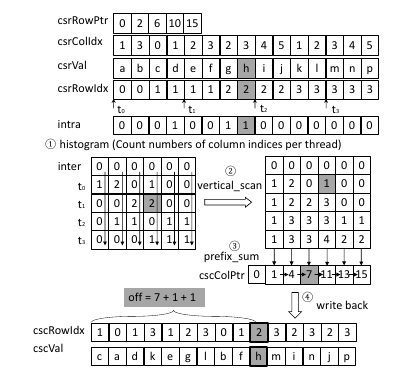
\includegraphics[scale=0.8]{scantrans.png}
		\label{scantrans}
		\caption{Scan Trans, esempio utilizzato in \cite{parallelTrans}.}
	\end{figure}
	
	\subsection{MergeTrans}
	L'algoritmo considerato prevede due passi importanti: \textit{sort} e \textit{merge}.
	Inizialmente sono stati creati gli indici di riga a partire dai puntatori delle colonne e su questi ultimi è stato fatto un sort su piccole porzioni di array, mantenendo quindi i vari blocchi disordinati tra di loro ma con gli elementi ordinati. Successivamente, utilizzando è stato il merge ricorsivo, partendo dai blocchi più piccoli, unendoli in blocchi sempre più grandi. Per funzionare questo processo necessita dell'utilizzo di due buffer di memoria che contengono gli elementi appena ordinati. Infine dai puntatori delle colonne vengono estretti gli indici e viene fatta la scan che ritorna il risultato in formato \textit{csc}. \newline
	Anche in questo caso le procedure utilizzate si trovano in sezione \ref{procedure}, e sono ordinatamente eseguite come segue:
	\begin{enumerate}
		\item pointers to index: \ref{pnt-to-idx},
		\item segmented sort: \ref{seg-sort},
		\item segmented merge: \ref{seg-merge},
		\item index to pointers: \ref{idx-to-pnt-merge},
		\item scan: \ref{scan}.
	\end{enumerate}
	
	\begin{figure}[H]
		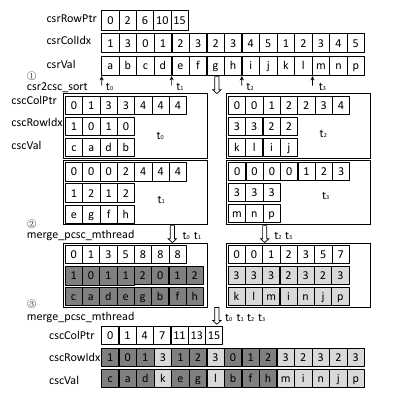
\includegraphics[scale=0.8]{mergetrans.png}
		\label{mergetrans}
		\caption{Merge Trans, esempio utilizzato in \cite{parallelTrans}.}
	\end{figure}
	

\section{Procedure Cuda}
\label{procedure}
% tutte le versioni x2 e x3
	In questa sezione vengono descritte le procedure Cuda principali che sono state utilizzate nelle implementazioni di \textit{Scan Trans} e \textit{Merge Trans}.

	\subsection{Pointers to index}
	\label{pnt-to-idx}
	Questa procedura prende in input l'array dei puntatori alle righe, e come dice il nome, crea un'array degli indici di riga. Quindi ad ogni thread viene assegnato un valore di \textit{csrRowPtr} e per ognuno di questi calcola inizio e fine e crea il nuovo array.
	
	\subsection{Index to pointers - Scan Trans}
	\label{idx-to-pnt-scan}
	Lo scopo di questa procedura è quello di trasfore l'array \textit{csrColIdx} in \textit{colPtr}. Esegue quindi il passo \circled{1} e \circled{2} in figura~\ref{scantrans}:
	\begin{enumerate}
		\item \textit{parallel histogram}: una thread per blocco(dimensione fissa) si occupa della costruzione degli array multidimensionali \textit{inter} e \textit{intra}. Quindi ogni blocco di thread prende un valore, e data la posizione all'interno di \textit{csrColIdx} salva nella posizione corretta i nuovi valori all'interno di inter e intra.
		\item \textit{vertical scan}: per ogni blocco verticale all'interno di \textit{inter} esegue una scan parallela e salva il risultato all'interno di una matrice chiamata \textit{colPtr}.
	\end{enumerate}

	\subsection{Reorder elements}
	\label{reoder-elem}
	Ogni thread si occupa di riordinare un blocco di elementi di dimensione fissa. Viene calcolato l'\textit{id} all'interno di \textit{csrColIdx}, dopodichè calcolata la posizione all'interno di \textit{csrColIdx}, \textit{inter} e \textit{intra} e viene posizionato il valore preso in \textit{cscRowIdx} e \textit{cscVal}. 
	Questa è l'ultima procedura che viene utilizzata in \textit{Scan Trans}, infatti si può notare che restituisce due array in formato csc.

	\subsection{Segmented sort}
	\label{seg-sort}
	Questa procedura, che chiama il relativo kernel, funziona passando come parametri un numero definito a priori (e.g. 128) che opera su blocchi di dimensione fissa anch'essi di $ len/n\_threads $, dove \textit{len} sta per nnz ovvero la dimensione di \textit{colIdx}.\newline
	Anche se il concetto è lo stesso la procedura viene divisa in due per semplificare il procedimento:
	\begin{itemize}
		\item \textit{segsort}: opera solamente su un array in input. Il kernel è stato sviluppato per funzionare con la \textit{shared memory}, quindi abbiamo un array temporaneo condiviso tra le thread. Ogni thread lavora su un elemento del blocco, priva vengono caricati i valori nella shared memory, poi viene trovata la posizione corretta all'interno dell'array non ordinato passato in input tenendo conto dei duplicati. Dopo aver trovato la posizione, il valore viene salvato nella posizione corretta all'interno della shared memory e infine salvato nel vettore di output-
		\item \textit{segsort3}: il concetto è lo stesso ma opera su 3 array in input.
	\end{itemize}
	
	\subsection{Segmented merge}
	\label{seg-merge}
	% TODO aspetta che cambia

	\subsection{Index to pointers - Merge Trans}
	\label{idx-to-pnt-merge}
	A differenza di \textit{index to pointers} per lo Scan Trans questa procedura utilizza solamente \textit{inter}, ma è sempre diviso in due:
	\begin{itemize}
		\item \textit{parallel histogram}: in questo caso abbiamo un numero di thread superiore rispetto al precedente(1024) che opera su una griglia di dimensione fissa. Allineo \textit{inter} sulla porzione di array che sto utilizzando trovando una dimensione costante del blocco ($ len/dimBlock $) e ogni thread dopo aver trovato il valore corretto all'interno dell'indice esegue una \textit{add atomica} sul valore trovato.
		\item \textit{vertical scan}: è lo stesso descritto in sezione \ref{idx-to-pnt-scan}\textit{-2}.
	\end{itemize}
	
	\subsection{Scan}
	\label{scan}
	% TODO è roba nostra?
	

\section{Benchmark}
\label{benchmark}
	Tutti i test sono stati effettuati sulle macchine locali e sul server Cuda01, quindi testati con diverse versioni di Cuda e come detto precedentemente anche di cuSPARSE. Le Gpu utilizzate sono:
	\begin{itemize}
		\item macchina locale:	% TODO che gpu?
		\item server cuda01:
	\end{itemize}
	Per la fase di test dell'implementazione sono state utilizzate principalmente due tipologie di matrici.
	
	\subsection{Matrici sparse casuali}
	A partire da dei valori fissi di \textit{m, n, nnz} è stata creata una matrice in formato Csr utilizzando come elementi dei valori generati in modo casuale compresi tra un minimo e un massimo a scelta. Come per i valori casuali, è possibile cambiare le dimensioni della matrice e passare dei nuovi valori all'eseguibile come descritto in sezione~\ref{applicativo-finale}.
	
	\subsection{Dataset utilizzato}
	In \cite{parallelTrans} è stato utilizzato un dataset di matrici sparse rappresentate in diversi formati. È stato fatto lo stesso anche nel nostro progetto, sono stati scaricati alcuni esempi presi da \cite{dataset}, e su questi sono stati eseguiti gli algoritmi implementati. Gli esempi tratti hanno varie dimensioni e il valore relativo all'elemento \textit{nnz} è solitamente un numero decimale. In sezione \ref{risultati} vegono mostrati gli esempi utilizzati e i rispettivi valori.
	

\section{Risultati}
	\label{risultati}
	% file csv
	% tabellone con speedup
	
	
\section{Conclusioni}
\label{conclusioni}
	% tirare le somme di cosa abbiamo ottenuto
	% cosa migliorare?
	% come possiamo continuare il progetto se avessimo avuto più tempo?
		% algo merge con merge buffer che è gia implementato
		% testare l'efficienza delle componenti rispetto alla implementazione nvidia
		% idx to pntrs (soffre race condition) --> un thread ha un blocco
		

\bibliographystyle{IEEEtran}
\bibliography{biblio}


%\appendix
%Se non avete abbastanza spazio, potete inserire le figure delle EFSM in una  pagina extra, appendice. Un esempio di come potete fare solo le Figure~\ref{fig:grande}, \ref{fig:piccola1}, \ref{fig:piccola2}.

\end{document}